\begin{frame}
  \frametitle{Results for the Previous Week}

  \begin{center}
    Here are the results for last week:

    \bigskip
    
    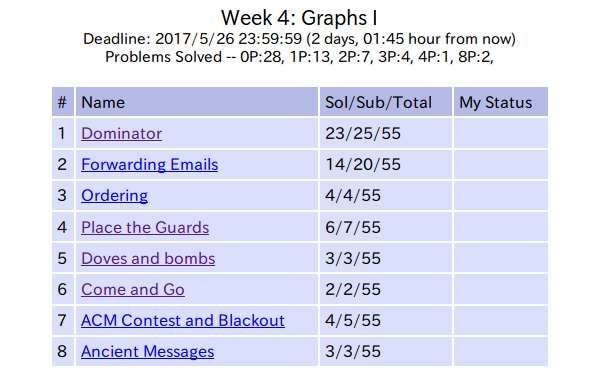
\includegraphics[width=0.8\textwidth]{img/resultsW4}

  \end{center}
\end{frame}

\begin{frame}
  \frametitle{Challenge Problem: Ancient Script}

  \begin{center}
    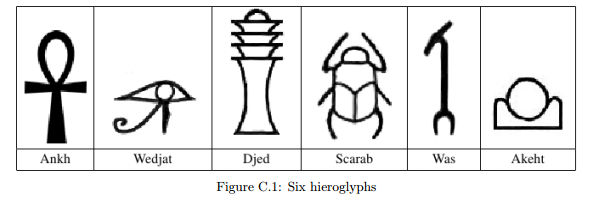
\includegraphics[width=0.8\textwidth]{img/symbols}
  \end{center}

  \bigskip
  
  \begin{itemize}
  \item The difference between the symbols is the number of holes!
  \item You can count the holes in a pixel image using {\bf connected
    components}
  \item Remove the connected component of ``outside'', then count
    the holes to know which symbols exist in the picture.
  \end{itemize}
\end{frame}

